% Szkielet dla pracy inżynierskiej pisanej w języku angielskim.

\documentclass[english,bachelor,a4paper,twoside]{ppfcmthesis}

\usepackage[utf8]{inputenc}
\usepackage[OT4]{fontenc}
\usepackage[T1]{fontenc}
\usepackage{graphicx}
\usepackage{listings}

\graphicspath{ {figures/} }

% Authors here.
\author{%
   Michał Kempka \album{105256} \and 
   Grzegorz Runc \album{109759} \and 
   Jakub Toczek \album{109704} \and 
   Marek Wydmuch \album{109746}}
\authortitle{}                                        % Do not change.
\title{VIZIA: 3D Video Game-based Environment for Research on Learning Agents from Raw Visual Information}        % Note how we protect the final title phrase from breaking (~zamiast spacyj)
\ppsupervisor{~Wojciech Jaśkowski,~Ph.~D.} % Your supervisor comes here.
\ppyear{2016}                                         % Year of final submission (not graduation!)

\begin{document}

% Front matter starts here
\frontmatter\pagestyle{empty}%
\maketitle\cleardoublepage%

% Blank info page for "karta dyplomowa"
\thispagestyle{empty}\vspace*{\fill}%
\begin{center}Tutaj przychodzi karta pracy dyplomowej;\\oryginał wstawiamy do wersji dla archiwum PP, w pozostałych kopiach wstawiamy ksero.\end{center}%
\vfill\cleardoublepage%

%Streszczenie i abstrakt
\chapter*{Streszczenie}
Zawartość streszczenia.

\chapter*{Abstract}
Abstract's content.

\cleardoublepage

% Table of contents.
\pagenumbering{Roman}\pagestyle{ppfcmthesis}%
\tableofcontents* \cleardoublepage%

% Main content of your thesis starts here.
\mainmatter%



\chapter{Introduction}
\label{ch:introduction}
\section{Motivation}


Visual signals are one of the main sources of information about the surrounding environment and are heavily relied by all humans and animals.
While computers have greatly exceeded humans in terms of raw data processing, they still do not match their ability to process images.
However, recent increase in computing power and emergence of affordable technologies allowing to perform general computations on graphics cards (CUDA, OpenCL) enabled a significant progress in this area.
An important part of this advance are deep convolutional neural networks (CNNs), which consist of multiple layers that analyse image on different levels of abstraction.


CNNs for the first time came into promience when were used to clasify 1.6 millions images into 1000 classes~\cite{NIPS2012_4824}.
This solution was so effective that now this is the prevalent method of image classification.
This succes hugely popularized CNNs and soon enough they were used for much more complex tasks.
In combination with reinforcement learning, they were used to model intellient agent which attempted playing 7 Atari 2600 games from Arcade Learning Platform\cite{mnih-atari-2013}.
In 6 of them the acheived results were better than in all of the previous approaches, and in the case of 3 results were better than those achievable by human players.
The main drawback of Atari games is that they are only two-dimensional, so their usability at solving real-world problems is quite limited, but reinforcement learning itself was successfully used for identifying features in static images \cite{conf/cvpr/GoodrichA12} and in robotics for controlling racing slot car using only image from the camera \cite{rieijcnn12} and even for steering RC helicopter\cite{Abbeel07anapplication}.

Bigger scope of practical applications is offered by 3D games which are a better approximation of the real-world.
Among 3D games, First Person Shooter (FPS) are interesting in particular becuase they offer simple and straightforward ways to implement rewarding mechanism, crucial in reinforcement learning.

FPS games have already been successfully used in research on artificial intelligence, especially the most popular ones such as Unreal Tournament \cite{6314567}, \cite{6922494} Counter-Strike \cite{5035619} or Quake III Arena \cite{el2007hybrid}.
However, in these studies agents acted upon high-level data which are normally inaccessible to human player like positions of all enemies, locations of item etc.
Supplying only raw visual information would relieve reaserchers of the burden of supplying AI high-level information and handcrafted features.
What is more it would force agents to become more autonomous and behave in a way more resembling real intelligent agents (humans and animals).
So far no studies have been conducted on the reinforcement learning from visual information obtained from 3D FPS games.


Currently there are no environments that allow using FPS games for research on artificial intelligence algorithms, in which agents could rely exclusively on raw visual information.
This could be a serious factor that is impending the progress of visual information-based research on reinforcement learning.
Engaging in that kind of research would require a large amount of work associated with creation of an environment integrating game engine with interface suited to reinforcement learning paradigm.
The existence of such a tool would allow to conduct experiments and focus on the goal of research without having to worry about availability of the test environments.
 

\section{Aims and scope}


The main aim of this thesis is to create easy to use and flexible environment for research on intelligent agents that work and learn using the raw visual information generated by the engine of 3D FPS game and conduct experiments that confirm the usability of the created environment.

The goal will be achieved by meeting the following objectives:
\begin{itemize}
 \item to compare and select needed technologies
 \item to implement environment
 \item to define and implement test scenarios in the created environment
 \item to select learning algorithms for deep neural networks
 \item to conduct experiments for simple test scenarios
\end{itemize}


The created environment should be based on opensource, lightweight 3D FPS game that allows total control over game's processing and customizing resolution and rendering parameters.
There should be implemented spectator mode, in which agent observes human playing.
Support for creation of custom scenarios should be essential part of the environment. 
Designed API should be reinforcement learning friendly and implemented in C++ with bindings to Python and possibly other languages (Java, Lua etc.)
The environment should be multiplatform, focused on Linux, with Windows and OS X support.
	
\section{Thesis organization}


This thesis is structured as follows. 
Chapter~\ref{chapter:architecture} gives an overview of technologies and tools used to develop the environment and describes environment's architecture. It addresses design decisions and problems and contains result of performance tests. 
Chapter~\ref{chapter:api} presents the designed application programming interface, python wrapper and shows API's usage examples. 
Chapter~\ref{chapter:scenarios} gives definition of scenario and presents tools and methods for creating scenarios. It contains the description of designed scenarios. 
Chapter~\ref{chapter:experiments} shows methods used for conducting experiments and their results. 
Chapter~\ref{chapter:conclusions} concludes this thesis and proposes directions for future work.

\section{Contributions}
	\subsection{Engineering Project}
	\begin{description}
		\item[Michał Kempka] \hfill
			\begin{itemize}
				\item part of interface design,
				\item testing and experiments,
				\item part of python binding,
				\item python examples,
				\item scenarios creation,
				\item support for configuration files.
			\end{itemize}
		\item[Grzegorz Runc] \hfill
			\begin{itemize}
				\item generation of depth buffer
				\item support for offscreen rendering
			\end{itemize}
		\item[Jakub Toczek] \hfill
			\begin{itemize}
				\item A
				\item B
				\item C
			\end{itemize}
		\item[Marek Wydmuch] \hfill
			\begin{itemize}
				\item Vizia API design
				\item Vizia API and ViziaDoomModule implementation
				\item CMake configuration
			\end{itemize}
	\end{description}
	
   	
	\subsection{Thesis}
	\begin{description}
		\item[Michał Kempka] \hfill
			\begin{itemize}
				\item foundations for Chapter \ref{ch:api},
				\item Chapter \ref{ch:scenarios},
				\item Chapter \ref{ch:experiment},
				\item Chapter \ref{ch:conclusions}.
			\end{itemize}
		\item[Grzegorz Runc] \hfill
			\begin{itemize}
				\item Chapter~\ref{ch:introduction}
				\item Section~\ref{sec:technologies}
			\end{itemize}
		\item[Jakub Toczek] \hfill
			\begin{itemize}
				\item A
				\item B
				\item C
			\end{itemize}
		\item[Marek Wydmuch] \hfill
			\begin{itemize}
				\item Section~\ref{sec:architecture}
				\item Section~\ref{sec:architecture_solutions}
				\item Section~\ref{sec:performance}
			\end{itemize}
	\end{description}


\chapter{Framework Architecture}

\section{Used Technologies}
What we used and why.
\begin{itemize}
\item zdoom, whole table with alternatives alternatives (full page)
\item linux focus, cpp core, python wrapper
\item acs scripting in doombuilder 2 for scenarios
\item python and lasagne for experiments
\end{itemize}

\section{Architecture}\label{sec:architecture}
	\begin{figure}
			\centering
			\includegraphics[scale=0.25]{architecture_diagram.png}
			\caption{Architecture of Vizia Environment.}\label{fig:architecture_diagram}
	\end{figure}

The main components of Vizia environament:
    \begin{itemize}
    \item Vizia library --- which provides a DoomGame API that allows user to configure, launch and play the game in several flow control modes.
    \item ViziaZDoom --- modified ZDoom engine with a Vizia module to communicate with a DoomGame object, control the game flow and adding additional rendering modes. It can act as a process under the control of the DoomGame object, Dome engine used for testing in Doom editors or as standalone process.
    \item Python and Java bindings - allowing the use of the DoomGame API in these languages.
    \end{itemize}


\subsection{The separate API and game processes}\label{sec:architecture_separate_processes}

When the user initiates the processing, the DoomGame object creates a second thread that starts ViziaZDoom process with the appropriate settings and supervises it. From this point the API and the game communicate using only a shared memory.


\subsection{Shared memory to communicate}\label{sec:architecture_shared_memory}

During initialization set of spaces are created in the shared memory space, which includes:
    \begin{itemize}
    \item A Pair of message queues to control the processing flow, and sending messages to the game.
    \item A Shared memory area  to exchange information about game input status. Both the API process and the game process reads and writes to shared memory.
    \item Shared memory areas where the game provides state of the game. These are the values of the variables games necessary to control the processing variables and a copy provided to you buffor wyrenderowanego in the game image. The game process saves to the memory, the process of API support.
    \end{itemize}
All shared memory spaces have unique names for each DoomGame object, which allows the coexistence of multiple instances.


\subsection{Vizia module inside ViziaZDoom}\label{sec:architecture_inside_viziazdoom}

Vizja module inside the engine initializes the shared memory to exchange information with this instance of the game. Then controls the flow of the game depending on the processing mode, and received messages and determines the following processing steps:

    \begin{itemize}
    \item Starting processing of the next game tic.
    \item Transmiting commands from the message queue to the game console.
    \item Sending inputu information from shared memory to the game console.
    \item Processing of events that the game window recieved since the last tic.
    \item Rendering the current frame.
    \item Updating the information about the current game state in the shared memory.
    \end{itemize}

\subsection{Flow control modes}\label{sec:architecture_modes}

The DoomGame API implements four flow control modes:
    
    \begin{itemize}
    \item Synchronous player
    \item Synchronous spectator
    \item Asynchronous player
    \item Asynchronous spectator
    \end{itemize}
    
    \subsubsection{Synchronous player mode}\label{sec:architecture_player_mode}
    
        \begin{figure}
			    \centering
			    \includegraphics[scale=0.25]{player_mode_diagram.png}
			    \caption{Processing flow in synchronous player mode.}\label{fig:player_mode_diagram}
	    \end{figure}
        
	    Synchronous player mode provides synchronous communication between the process that uses the API and the game process. It allows AI agent to make actions as a player. 
	    
	    In this mode, the API and the game processes communicates every tic and are waiting for each other. The game process waits until the API sends a message requesting processing of the next tic and optional update. The game process, after receiving the message, sends input information (AI agent's action) to the game console, process next game tic, and if update was requested renders the current frame and updates the information about the current game state in the shared memory. After this the game process sends a message about completing request and starts waiting for the message processing of the next tic. The process that uses the API waits for the message about completing request.
	    
	    This mode is designed for the singleplayer, the multiplayer will not work correctly - the game net code is disabled in this mode.

    \subsubsection{Synchronous spectator mode}\label{sec:architecture_spectator_mode}

	    \begin{figure}
			    \centering
			    \includegraphics[scale=0.25]{spectator_mode_diagram.png}
			    \caption{Processing flow in synchronous spectator mode.}\label{fig:spectator_mode_diagram}
	    \end{figure}
	    
	    Synchronous spectator mode provides synchronous communication between the process that uses the API and the game process. It allows AI agent to observe a human player's actions. 
	    
	    In this mode the API and the game processes communicates every tic and are waiting for each other. The game process waits until the API sends a message requesting processing of the next tic and optional update. The game process, after receiving the message, process the window input events that have taken place since the last update request (last human player's action), updates the input information in the shared memory, process next game tic and if update was requested renders the current frame and updates the information about the current game state in the shared memory. After this the game process sends a message about completing request and starts waiting for the message processing of the next tic. The process that uses the API waits for the message about completing request.

        Before processing of the next game tic the delay may be introduced in order to ensure the maximum processing speed of 35 tics per second (designed Doom ticrate).
        
        This mode is designed for the singleplayer, the multiplayer will not work correctly - the game network code is disabled in this mode.

    \subsubsection{Asynchronous player mode}\label{sec:architecture_async_player_mode}

	    \begin{figure}
			    \centering
			    \includegraphics[scale=0.25]{async_player_mode_diagram.png}
			    \caption{Processing flow in asynchronous player mode.}\label{fig:async_player_mode_diagram}
	    \end{figure}
	    
	    Asynchronous player mode provides asynchronous communication between the process that uses the API and the game process. It allows AI agent to make actions as a player. 
	    
	    In this mode, the game process continuously process the game tics a constant speed of 35 tics per second (designed Doom ticrate) without waiting for the API process. The API can send a message requesting update. Before each tic the game process checks if it received a message requesting update. After receiving such the message, it sends the input information (AI agent's action) to the game console, process next game tic, updates the information about the current game state in the shared memory, sends a message about completing request and continues processing of the game tics. The process that uses the API waits for the message about completing request.
	    
	    In this mode, both the singleplayer as well as the multiplayer will work correctly - the game network code is disabled in this mode.

    \subsubsection{Asynchronous spectator mode}\label{sec:architecture_async_spectator_mode}

	    \begin{figure}
			    \centering
			    \includegraphics[scale=0.25]{async_spectator_mode_diagram.png}
			    \caption{Processing flow in asynchronous spectator mode.}\label{fig:async_spectator_mode_diagram}
	    \end{figure}
	    
	    Asynchronous spectator mode provides asynchronous communication between the process that uses the API and the game process.It allows AI agent to observe a human player's actions. 
	    
	    In this mode, the game process continuously process the game tics at a constant speed of 35 tics per second (designed Doom ticrate) without waiting for the API process. The API can send a message requesting update. Before each tic the game process checks if it received a message. After receiving such the message, it updates the input information in the shared memory (last human player's action), process next game tic, updates the information about the current game state in the shared memory, sends a message about completing request and continues processing of the game tics. The process that uses the API waits for the message about completing request.

        In this mode processing of the window input events and rendering is performed in each tic.
        
        In this mode, both the singleplayer as well as the multiplayer will work correctly.

\section{Explanation of problems and solutions}\label{sec:architecture_solutions}

\subsubsection{Why separate doom executable?}

Doom engine was designed as standalone executable. It has a diffrent entry point for every operating system and a lot of exit points what makes it difficult to pack it inside library without making any fundamental changes in it's code, in addition, this approach would not give any additional benefits. Also, leaving the Doom engine as a separate executable allows to use it with Doom editors and as standalone Doom engine for testing scenarios.

\subsubsection{Why shared memory to communicate?}

Shared memory is the fastest way to transfer large amounts of data and allows to use this data witout additional copying and processing. 
Because the game process uses shared memory only at the API request (and the API is waiting for completion of it) additional access control mechanism is not needed.

\subsubsection{Zbuffer}

Zostawiam Ci to Grzesiu. //TO DO

\subsubsection{Why multiplayer will not work in synchronous modes?}

Doom engine uses a peer-to-peer communication in multiplayer and requires tight synchronization between all game clients based on real time.
In synchronous modes time when next tic will be processed is unknown - too slow or too fast processing leads to synchronization and unpredictable behaviors and errors in processing. Therefore, the game network code has been disabled in synchronous modes.

\subsubsection{Why OSX is not supported?}

All Vizia environment code is OSX compatible. Due to the lack of access to OSX machine developers have not tested build system for it.

\subsubsection{Why game and scenario files are separated?}

Doom engine uses diffrent type of files for storing data and resources. (WAD and PK3 files) It allows to load main game resources from one file and many additional (scenario) resources from separate files. 

\section{Performance}
Table with some fps ratings and a graph.
Conclusions: it's fast enough, any reasonably good AI will be much slower during learning process.





\chapter{Application Programming Interface}
\section{Methods}
	\subsection{Configuration}
	Methods described below are setting the main parameters of the environment, such as resolution of the generated image or Intelligent Agent's available actions. They should be invoked before the init() method. Any attempt to invoke them after initialization will result in a warning/exception depending on severity of consequences. 
	\vspace{20pt}

		\begin{clinee}
		DoomGame();
		\end{clinee}

Constructor that creates an instance of the game. Zdoom is not ready for action after the constructor, it needs further initialization. Object is inicialized with the following values:
	\begin{itemize}
\item Resolution: 640x480
\item Game path: ./viziazdoom
\item Game iwad path: "./doom2.wad"
\item Map: map01 (first map created in the iwad file if it's not changed purposefully)
\item Mode: PLAYER
\item GameVariables: none
\item CustomGameArg: none
\item Available buttons: ATTACK, USE, JUMP, CROUCH, SPEED, MOVE\_RIGHT, MOVE\_LEFT, MOVE\_BACKWARD, MOVE\_FORWARD, TURN\_RIGHT, TURN\_LEFT
\item Rendering: All
\item Window: displayed 
\item DoomSkill: ??????????
\item Co z tymi autostartami i rewardami?
	\end{itemize}


\vspace{20pt}
\begin{clinee}
~DoomGame();
\end{clinee}

The destructor that safely ends the work of environment and removes the object.


\vspace{20pt}
\begin{clinee}
bool init();
\end{clinee}

Function which initializes enviroment. Configuration cannot be changed after invokation of init(). Dooms instance is created in separate process. Returns true when game was started properly. 


\vspace{20pt}
\begin{clinee}
bool loadConfig(std::string filename);
\end{clinee}

Loads and sets configuration from a configuration file. It's syntax is better described in Section~\ref{sec:configuration_file}. The configuration file can substitute any combination of the following methods call. In case of multiple invokations, they will overwrite selected settings from previous calls. Return true when all configuration was read properly.


\vspace{20pt}
\begin{clinee}
void addAvailableButton(Button button);
\end{clinee}

Adds support for the specified actions (e.g. TURN\_LEFT, MOVE\_FORWARD ). If no buttons are specified (the method is not called) 11 default buttons are added. Their list may be found in constructor description.


\vspace{20pt}
\begin{clinee}
void addAvailableButton(Button button, int maxValue);
\end{clinee}

Adds support for the specified actions responsible for rotation and sets the amount of movement done. It only applies to "buttons" responsible for rotation. it effectively constraints rotation speed. %TODO CO TO ROBI?!


\vspace{20pt}
\begin{clinee}
void setButtonMaxValue(Button button, int maxValue);
\end{clinee}

Sets the button's max value. It only applies to "buttons" responsible fors rotation and moving(with specified speed), it effectively constraints rotation/moving speed.
0 means no constraint and it's the default behavior TODO %TODO CO TO ROBI?!


\vspace{20pt}
\begin{clinee}
void addAvailableGameVariable(GameVariable var);
\end{clinee}

Adds given GameVariable to the list of values returned in getState() (e.g. AMMO1, HEALTH, ATTACK\_READY).


\vspace{20pt}
\begin{clinee}
void clearAvailableButtons();
\end{clinee}

Disables support for any specified buttons. It will result in default setting which can be found in constructor description.


\vspace{20pt}
\begin{clinee}
void clearAvailableGameVariables();
\end{clinee}

Clears the list of game variables returned in getState().


\vspace{20pt}
\begin{clinee}
void addCustomGameArg(std::string arg);
\end{clinee}

Adds a custom argument for the zdoom process. %TODO OPIS


\vspace{20pt}
\begin{clinee}
void clearCustomGameArgs();
\end{clinee}

Clears all arguments specified by addCustomGameArg().


\vspace{20pt}
\begin{clinee}
void setMode(Mode mode);
\end{clinee}

Sets mode in which the game will be started. Supported formats are defined in Mode enumaration (e.g. PLAYER, SPECTATOR).


\vspace{20pt}
\begin{clinee}
void setDoomGamePath(std::string path);
\end{clinee}

Sets path to zdoom executable.


\vspace{20pt}
\begin{clinee}
void setDoomIwadPath(std::string path);
\end{clinee}

Sets path to the game iwad file.


\vspace{20pt}
\begin{clinee}
void setDoomFilePath(std::string path);
\end{clinee}

Sets path to additional iwad file (e.g. scenario).


\vspace{20pt}
\begin{clinee}
void setDoomMap(std::string map);
\end{clinee}

Sets map to be used by doom.


\vspace{20pt}
\begin{clinee}      
void setDoomSkill(int skill);
\end{clinee}

Sets doom game difficulty level (0-5) which is called skill in doom. Less means easier. It affects ammo, life amount and monster aggressiveness. %TODO co tutaj? 


\vspace{20pt}
\begin{clinee}
void setDoomConfigPath(std::string path);
\end{clinee}

Sets path for doom configuration file.


\vspace{20pt}
\begin{clinee}    
void setEpisodeStartTime(unsigned int tics);
\end{clinee}

Sets start delay of every episodes in doom tics. Every episode will effectively start (from the user's perspective) after given number of tics.


\vspace{20pt}
\begin{clinee}
void setEpisodeTimeout(unsigned int tics);
\end{clinee}

Sets quantity of tics after which the episode will be finished.


\vspace{20pt}
\begin{clinee}
void setLivingReward(double livingReward);
\end{clinee}

Sets the reward granted for player being alive after each tic.


\vspace{20pt}
\begin{clinee}
void setDeathPenalty(double deathPenalty);
\end{clinee}

Sets penalty for player's death. In case of negative value, player will be rawarded for each decease.


\vspace{20pt}
\begin{clinee}
void setAutoNewEpisode(bool set);
\end{clinee}

Determines if automatic episode restart will be set in case of the end of previous one.


\vspace{20pt}
\begin{clinee}
void setNewEpisodeOnTimeout(bool set);
\end{clinee}

Determines if automatic episode restart will be set in case of the timeout.


\vspace{20pt}
\begin{clinee}
void setNewEpisodeOnPlayerDeath(bool set);
\end{clinee}

Determines if automatic episode restart will be set in case of players death.


\vspace{20pt}
\begin{clinee}
void setNewEpisodeOnMapEnd(bool set);
\end{clinee}

Determines if automatic episode restart is set when player reaches the end of the map.


\vspace{20pt}
\begin{clinee}
void setScreenResolution(ScreenResolution resolution);
\end{clinee}

Sets screen resolution. Supported resolutions are part of ScreenResolution Enumeration type and their format is: RES\_xXy (e.g. RES\_320X240, RES\_1920X1080). Buffer as well as content of zdoom's window is affected.


\vspace{20pt}
\begin{clinee}
 void setScreenFormat(ScreenFormat format);
\end{clinee}

Sets format of the screen buffer. Supported formats are defined in ScreenFormat enumaration (e.g. CRCGCB, RGB24, GRAY8). Content displayed in zdoom's window what change no matter which format you choose - it only affects the buffer.


\vspace{20pt}
\begin{clinee}       
void setRenderHud(bool hud);
void setRenderWeapon(bool weapon);
void setRenderCrosshair(bool crosshair);
void setRenderDecals(bool decals);
void setRenderParticles(bool particles);
\end{clinee}

Methods that determine if some elements (hud, weapon, crosshair, decals, particles) will be displayed.


\vspace{20pt}
\begin{clinee}
void setWindowVisible(bool visibility);
\end{clinee}

Determines if zdoom's window will be visible.
Turning it off will result in:
\begin{itemize}
\item Linux - rendering and any computations connected with the window will be skipped. It results in processing acceleration
\item Windows - window will be hided. No processing acceleration
\end{itemize}


\vspace{20pt}
\begin{clinee}
void setConsoleEnabled(bool console);
\end{clinee}

Determines if zdoom's and vizia's console output will be displayed (e.g. "You picked up a medpack", "Player killed himself.", "Vizia\_init ....")


\vspace{20pt}
\subsection{Runtime}
The following methods handles gameplay. They directly affect the game and should be used after inicialization. 
Any attempt to invoke them before it will result in a warning/exception depending on severity of consequences. 


\vspace{20pt}
\begin{clinee}
void newEpisode();
\end{clinee}

Initializes new episode. All rewards, map state etc are restarted.


\vspace{20pt}
\begin{clinee}
	void setAction(std::vector<int> &actions);
\end{clinee}

Sets the player's behavior in the next tic.
Each vector's value corresponds to button specified with addAvailableButton() function (in invocation order).
In case of possitive value, picked action will be triggered with the specified strength. Descrete actions (e.g. ATTACK) will be performed once.


\vspace{20pt}
\begin{clinee}
	void advanceAction();
\end{clinee}

Method performs a tic using action obtained by setAction(). After function call, action vector is not reseted and will be performed once again if not changed.


\vspace{20pt}
\begin{clinee}
	void advanceAction(bool stateUpdate, bool renderOnly, unsigned int tics);
\end{clinee}

Method performs a given number of tic in the row. Descrete actions (e.g. ATTACK) will be only performed in the first tic, analog actions (moving, turning) will be repeated every tic. 
Function also determines if state should be updated. What's more, setting renderOnly option as true will disable buffer update. Hovewer, it will not affect zdoom main window.  


\vspace{20pt}
\begin{clinee}
	double getLastReward();
\end{clinee}

Returns the reward from last advanceAction. If a single action lasted longer then one tick, function it will return cumulative reward from all tics.


\vspace{20pt}
\begin{clinee}
	double makeAction(std::vector<int> &actions);
\end{clinee}

Function combining usibility of setAction(), advanceAction() and getLastReward(). It sets the player's behavior in the next tic, performe one and returns reward.
Each vector's value corresponds to button specified with addAvailableButton() function (in invocation order).
In case of possitive value, picked action will be triggered with the specified strength. Descrete actions (e.g. ATTACK) will be performed once. 


\vspace{20pt}
\begin{clinee}
	double makeAction(std::vector<int> &actions, unsigned int tics);
\end{clinee}

Function combining usibility of setAction(), advanceAction() and getLastReward(). It sets the player's behavior in the next number of tics given to the function, performes it and returns cumulative reward from all tics. Each vector's value corresponds to button specified with addAvailableButton() function (in invocation order). Descrete actions (e.g. ATTACK) will be only performed in the first tic, analog actions (moving, turning) will be repeated every tic with given strength.
State will be updated after that. Buffer will not be updated.


\vspace{20pt}
\begin{clinee}
	State getState();
\end{clinee}

Returns struct State with the current game state. More detailed description of the struct can be found in Section~\ref{sec:structs}.


\vspace{20pt}
\begin{clinee}
	std::vector<int> getLastAction();
\end{clinee}

Returns a vector with the last action performed. Each vector's value corresponds to button specified with addAvailableButton() function (in invocation order). Most usefull in SPECTATOR mode.


\vspace{20pt}
\begin{clinee}
	uint8_t * const getGameScreen();
\end{clinee}

Returns the screen buffer. Values depend on the settings set befor inicialization. The same value may be found in State structure. Its length is returned in getScreenPitch() function.


\vspace{20pt}
\begin{clinee}
	int getGameVariable(GameVariable var);
\end{clinee}

Returns value of the specified game variable (AMMO1, HEALTH etc.). It does not need to be a value returned in State.
It could be used for e.g. shaping. Returns 0 in case of not finding given GameVariable.


\vspace{20pt}
\begin{clinee}
	double getSummaryReward();
\end{clinee}

Returns sum of all rewards gathered in the current episode.


\vspace{20pt}
\begin{clinee}
	bool isNewEpisode();
\end{clinee}

Checks if the current episode is in the initial state. Returns true if no tic was performed.


\vspace{20pt}
\begin{clinee}
	bool isEpisodeFinished();
\end{clinee}

Checks if the current episode is in the terminal state. Returns true if the episode has ended. No makeAction/advanceAction functions should be called after this point.


\vspace{20pt}
\begin{clinee}
	void setSeed(unsigned int seed);
\end{clinee}

Sets the seed of the randomizing engine. Using the same seed and actions in another episode will affect in reproducing the gameplay.


\vspace{20pt}
\begin{clinee}
	void close();
\end{clinee}

Closes zdoom engine and corresponding processes. Metod frees used resources (memory allocations e.t.c). It is automatically invoked by destructor - should be used only when closing zdoom engine in the middle of processing is needed.


\vspace{20pt}
\begin{clinee}
	bool isRunning();
\end{clinee}

Checks if the current zdoom process is running.


\vspace{20pt}
\begin{clinee}
	void sendGameCommand(std::string cmd);
\end{clinee}

Sends a given command to zdoom console. Can be used for cheats, multiplayer e.t.c.


\vspace{20pt}
\subsection{QUERY INTERFACE}


Api provides a number of getters associated with the above-mentioned functions and a set of additional methods to help converts units.
  

\vspace{20pt}
\begin{clinee}
int getAvailableButtonsSize();
int getAvailableGameVariablesSize();
Mode getMode();
double getLivingReward();
double getDeathPenalty();
unsigned int getEpisodeStartTime();
unsigned int getEpisodeTimeout();
unsigned int getEpisodeTime();
int getScreenWidth();
int getScreenHeight();
int getScreenChannels();
size_t getScreenPitch();
size_t getScreenSize();
ScreenFormat getScreenFormat();
unsigned int getSeed();
int getButtonMaxValue(Button button);
\end{clinee}


\paragraph {Metods} Metods outsite the DoomClass:


\begin{clinee}
unsigned int DoomTics2Ms(unsigned int tics);
\end{clinee}

Function calculating number of milliseconds during given tics.


\vspace{20pt}
\begin{clinee}
unsigned int Ms2DoomTics(unsigned int ms);
\end{clinee}

Function calculating how many tics will be made during given number of milliseconds.


\vspace{20pt}
\begin{clinee}
double DoomFixedToDouble(int doomFixed);
\end{clinee}

DO OPISANIA


\vspace{20pt}
\section{Structures and Enumerations} \label{sec:structs}
\subsection{State}


Structure created to store all the information needed by inteligent agent to process the image.  
It is composed of three public fields:

\vspace{20pt}	
\begin{clinee}
	struct State {
	    unsigned int number; 
	    std::vector<int> gameVariables;
	    uint8_t * imageBuffer;
	};
\end{clinee}
number - Number of the state in the current episode. (tic number?)\\
gameVariables - vector storing user-defined, during the configuration, values drawn from the game such as AMMO or HEALTH 
imageBuffer - pointer to the screen buffer, containing the image information.
\begin{itemize}
\item struct state
\item enumeration types . . .or maybe move it to the apendinx?
\end{itemize}
\subsection{Mode}
Enumeration used to set the general game mode.
Posible values:
\begin{itemize}
\item PLAYER - 
\item SPECTATOR -
\item ASYNC\_PLAYER -
\item ASYNC\_SPECTATOR -
\end{itemize}
\subsection{ScreenFormat}
Enumeration used to set the general game mode.
\begin{itemize}
 \item CRCGCB 
 \item CRCGCBZB
 \item RGB24
 \item RGBA32
 \item ARGB32
 \item CBCGCR
 \item CBCGCRZB
 \item BGR24
 \item BGRA32
 \item ABGR32
 \item GRAY8
 \item ZBUFFER8
 \item DOOM\_256\_COLORS
\end{itemize}
\subsection{ScreenResolution}
\begin{itemize}
\item RES\_40X30,
 \item      RES\_60X45,
 \item       RES\_80X50,
 \item       RES\_80X60,
 \item       RES\_100X75,
 \item       RES\_120X75,
 \item       RES\_120X90
 \item       RES\_160X100,
 \item      RES\_160X120,
      \item  RES\_200X120,
      \item  RES\_200X150,
      \item  RES\_240X135,
      \item  RES\_240X150,
      \item  RES\_240X180,
      \item  RES\_256X144,
      \item  RES\_256X160,
      \item  RES\_256X192,
      \item  RES\_320X200,
      \item  RES\_320X240,
      \item  RES\_400X225,	// 16:9
      \item  RES\_400X300,
  \item      RES\_480X270,	// 16:9
 \item       RES\_480X360,
 \item       RES\_512X288,	// 16:9
 \item       RES\_512X384,
 \item       RES\_640X360,	// 16:9
 \item       RES\_640X400,
 \item       RES\_640X480,
 \item       RES\_720X480,	// 16:10
 \item       RES\_720X540,
 \item       RES\_800X450,	// 16:9
 \item       RES\_800X480,
 \item       RES\_800X500,	// 16:10
  \item      RES\_800X600,
 \item       RES\_848X480,	// 16:9
 \item       RES\_960X600,	// 16:10
 \item       RES\_960X720,
 \item       RES\_1024X576,	// 16:9
 \item       RES\_1024X600,	// 17:10
 \item       RES\_1024X640,	// 16:10
 \item       RES\_1088X612,	// 16:9
 \item       RES\_1152X648,	// 16:9
 \item       RES\_1152X720,	// 16:10
 \item       RES\_1152X864,
 \item       RES\_1280X720,	// 16:9
 \item       RES\_1280X854,
 \item       RES\_1280X800,	// 16:10
 \item       RES\_1280X960,
 \item       RES\_1280X1024,	// 5:4
 \item       RES\_1360X768,	// 16:9
 \item       RES\_1366X768,
 \item       RES\_1400X787,	// 16:9
 \item       RES\_1400X875,	// 16:10
 \item       RES\_1400X1050,
 \item       RES\_1440X900,
 \item       RES\_1440X960,
 \item       RES\_1440X1080,
  \item      RES\_1600X900,	// 16:9
 \item       RES\_1600X1000,	// 16:10
 \item       RES\_1600X1200,
 \item       RES\_1680X1050,	// 16:10
 \item       RES\_1920X1080,
 \item       RES\_1920X1200,
 \item       RES\_2048X1536,
 \item       RES\_2560X1440,
 \item       RES\_2560X1600,
 \item       RES\_2560X2048,
 \item       RES\_2880X1800,
 \item       RES\_3200X1800,
  \item      RES\_3840X2160,
 \item       RES\_3840X2400,
 \item       RES\_4096X2160,
  \item      RES\_5120X2880,
\end{itemize}
\subsection{GameVariable}
\begin{itemize}
\item KILLCOUNT,
\item        ITEMCOUNT,
\item        SECRETCOUNT,
\item        FRAGCOUNT,
\item        HEALTH,
\item        ARMOR,
\item        DEAD,
\item        ON\_GROUND,
\item        ATTACK\_READY,
\item        ALTATTACK\_READY,
 \item       SELECTED\_WEAPON,
\item      SELECTED\_WEAPON\_AMMO,
 \item       AMMO0,
\item        AMMO1,
\item        AMMO2,
\item        AMMO3,
 \item       AMMO4,
 \item       AMMO5,
 \item       AMMO6,
 \item       AMMO7,
\item       AMMO8,
\item        AMMO9,
 \item       WEAPON0,
 \item       WEAPON1,
\item        WEAPON2,
 \item       WEAPON3,
 \item       WEAPON4,
 \item       WEAPON5,
\item        WEAPON6,
\item        WEAPON7,
\item        WEAPON8,
\item        WEAPON9,
 \item       USER1,
 \item       USER2,
 \item       USER3,
 \item       USER4,
 \item       USER5,
\item        USER6,
\item        USER7,
\item        USER8,
\item        USER9,
\item        USER10,
\item        USER11,
\item        USER12,
\item        USER13,
\item        USER14,
\item        USER15,
\item        USER16,
\item        USER17,
\item        USER18,
\item        USER19,
\item        USER20,
\item        USER21,
\item        USER22,
\item        USER23,
\item        USER24,
\item        USER25,
\item        USER26,
\item        USER27,
\item        USER28,
\item        USER29,
\item        USER30,
\end{itemize}
\subsection{Button}
\begin{itemize}
\item ATTACK = 0,
\item         USE = 1,
\item         JUMP = 2,
\item         CROUCH = 3,
\item         TURN180 = 4,
\item         ALTATTACK = 5,
\item         RELOAD = 6,
\item         ZOOM = 7,

\item         SPEED = 8,
\item         STRAFE = 9,

\item         MOVE\_RIGHT = 10,
\item         MOVE\_LEFT = 11,
\item         MOVE\_BACKWARD = 12,
\item         MOVE\_FORWARD = 13,
\item         TURN\_RIGHT = 14,
\item         TURN\_LEFT = 15,
\item         LOOK\_UP = 16,
\item         LOOK\_DOWN = 17,
\item         MOVE\_UP = 18,
\item         MOVE\_DOWN = 19,
\item         LAND = 20,
        //SHOWSCORES 20

\item         SELECT\_WEAPON1 = 21,
\item         SELECT\_WEAPON2 = 22,
\item         SELECT\_WEAPON3 = 23,
\item         SELECT\_WEAPON4 = 24,
\item         SELECT\_WEAPON5 = 25,
\item         SELECT\_WEAPON6 = 26,
\item         SELECT\_WEAPON7 = 27,
\item         SELECT\_WEAPON8 = 28,
\item         SELECT\_WEAPON9 = 29,
 \item        SELECT\_WEAPON0 = 30,

\item     SELECT\_NEXT\_WEAPON = 31,
 \item        SELECT\_PREV\_WEAPON = 32,
\item         DROP\_SELECTED\_WEAPON = 33,

 \item        ACTIVATE\_SELECTED\_ITEM = 34,
 \item        SELECT\_NEXT\_ITEM = 35,
 \item        SELECT\_PREV\_ITEM = 36,
 \item        DROP\_SELECTED\_ITEM = 37,

 \item        LOOK\_UP\_DOWN\_DELTA = 38,
 \item        TURN\_LEFT\_RIGHT\_DELTA = 39,
 \item        MOVE\_FORWARD\_BACKWARD\_DELTA = 40,
 \item        MOVE\_LEFT\_RIGHT\_DELTA = 41,
 \item        MOVE\_UP\_DOWN\_DELTA = 42,
\end{itemize}
\section{Configuration file}\label{sec:configuration_file}


Configuration file stores group of parameters and initial settings for the future use. It can be loaded into the game before inicialization. Settings can be overwritten after that action, giving the possibility of changing sigle parameter without interference in the file itself. There should be met certain requirements as to its content and name to make it load successfully.

Name of the configuration file should be with .properties suffix.

Content of the file should be composed of keywords identifying the setting and the value assigned to it separated with '='. Keyword is constructed similarly to the setting name, for example: episodeStartTime, windowVisible. However, two of them differ: availablebuttons, availablegamevariables.
Keyword can be written in both underscore and camel notation (case-insensitive). 


Value should be placed after '=' sign. File paths should not be placed between "" marks like the rest of the string values.
\begin{cblock}
...
#Values
living_reward = -1
render_crosshair = false
#Path
doom_iwad_path = ../../scenarios/doom2.wad
doom_file_path = ../../scenarios/basic.wad
#Normal String
doom_map = "map01"
...
\end{cblock}
Enum values should be passed using their name.
\begin{cblock}
...
#Enums
screen_format = CRCGCB
mode = PLAYER
...
\end{cblock}
Each setting should be separated from each other by a sign of the new line. In order to improve readability, it's possible to add a comment line by adding a '\#' sign at the beginning of the new line.

An exceptionally behave here availablebuttons and availablegamevariables functions because instead of individual variables, take as an argument the list of values in '\{\}'. The individual components should be separated from each other by a newline.
\begin{cblock}
...
# Available buttons
available_buttons = 
	{ 
		MOVE_LEFT 
		MOVE_RIGHT 
		ATTACK 
	}
# Game variables that will be in the state
available_game_variables = { AMMO2}
...
\end{cblock}

\section{Wrappers}
\subsection{Python}

Python functions and metods are very similar to the c++ ones. Howewer, because of the language differences, some of the values may vary. All differences are listed below.

\paragraph {Naming}
Naming convention used in python binding is underscore. The only exception is the constructor which is named in the same way like in c++.

\begin{cblock}
c++: DoomFixedToDouble(int doomFixed)
python: doom_fixed_to_double(int doomFixed)
\end{cblock}


\paragraph {Structures}
 State is changed structuraly: bufer is a numpy array and game variables are contained in a Python list. Whats more, getState() copies the buffer and gameVariables what doesn't happen in cpp. 
\paragraph {Enumerations}
Python equivalent of enums were created with the same names.
\paragraph {Types}
Due to the languages differences, some types have been modified.
\begin{itemize} 
\item Vectors in all functions were changed to python lists of compatible type.

\item  uint8\_t, unsigned int, size\_t were changed to int
\end{itemize}



\subsection{Java}
Java, like python, is a bit different then c++. All differences and the most important principles of using are listed below.

\paragraph {Naming}
 Naming convention is camelcase 
\begin{clinee}
c++: DoomFixedToDouble(int doomFixed)
java: DoomFixedToDouble(int doomFixed)
\end{clinee}
\paragraph {Structures}
State is changed structuraly: bufer and game variables are int tables (int[]). Whats more, getState copies the buffer and gameVariables, it doesn't happen in cpp. 
\paragraph {Enumerations}
 Enumerations were created the same like in c++ (you have to use them like in java:)
\begin{clinee}
 dg.addAvailableButton(Button.ATTACK);
\end{clinee}
\paragraph {Types}
Due to the languages differences, some types have been modified.
\begin{itemize}
\item Vectors in all functions were changed to java tables of compatible type (vector<int> = int[]).
\item uint8\_t, unsigned int, size\_t were changed to int
\end{itemize}
\section{Extended Examples}

\chapter{Scenarios}\label{ch:scenarios}

To allow researchers to evaluate learning agents in conditions of different characteristics, VIZIA provides a mechanism of scenarios.

This chapter defines what a scenario is (see Section \ref{sec:scenario_definition}), describes sample scenarios provided with VIZIA (see Section \ref{sec:scenarios}) and points out essentials of creating custom scenarios (see Section \ref{sec:creating_scenarios}).

\section{Definition}\label{sec:scenario_definition}
	Scenarios are DOOM resource files in special WAD format. A single scenario defines a map (structure of the world e.g. walls, corridors, monsters) and~a~script which determines behavior of entities and events. The script is also the place to assign rewards for various events. A scenario can define multiple maps in one WAD file and~they all can be accessed by VIZIA API. Default name for a map is `map01' but in general it can be completely arbitrary. Each map requires a separate script file.
	\\
	Scenarios do not affect:
	\begin{itemize}
		\item constraints regarding buttons that can and cannot be used,
		\item episode timeout,
		\item skill level (they can affect; however, behaviors that depend on it), and
		\item any rendering options e.g. screen resolution or~crosshair visibility.
	\end{itemize}

	Due to scenarios' ability to set rewards they could be used to implement a~reward for staying alive and a~penalty for dying. Nonetheless, using API's \emph{setLivingReward} and \emph{setDeathPenalty} methods is the preferred way to achieve this(see Section \ref{subsec:config_methods} and \ref{sec:configuration_file}) .

\section{Tools}\label{sec:tools}
	\begin{figure}
			\centering
			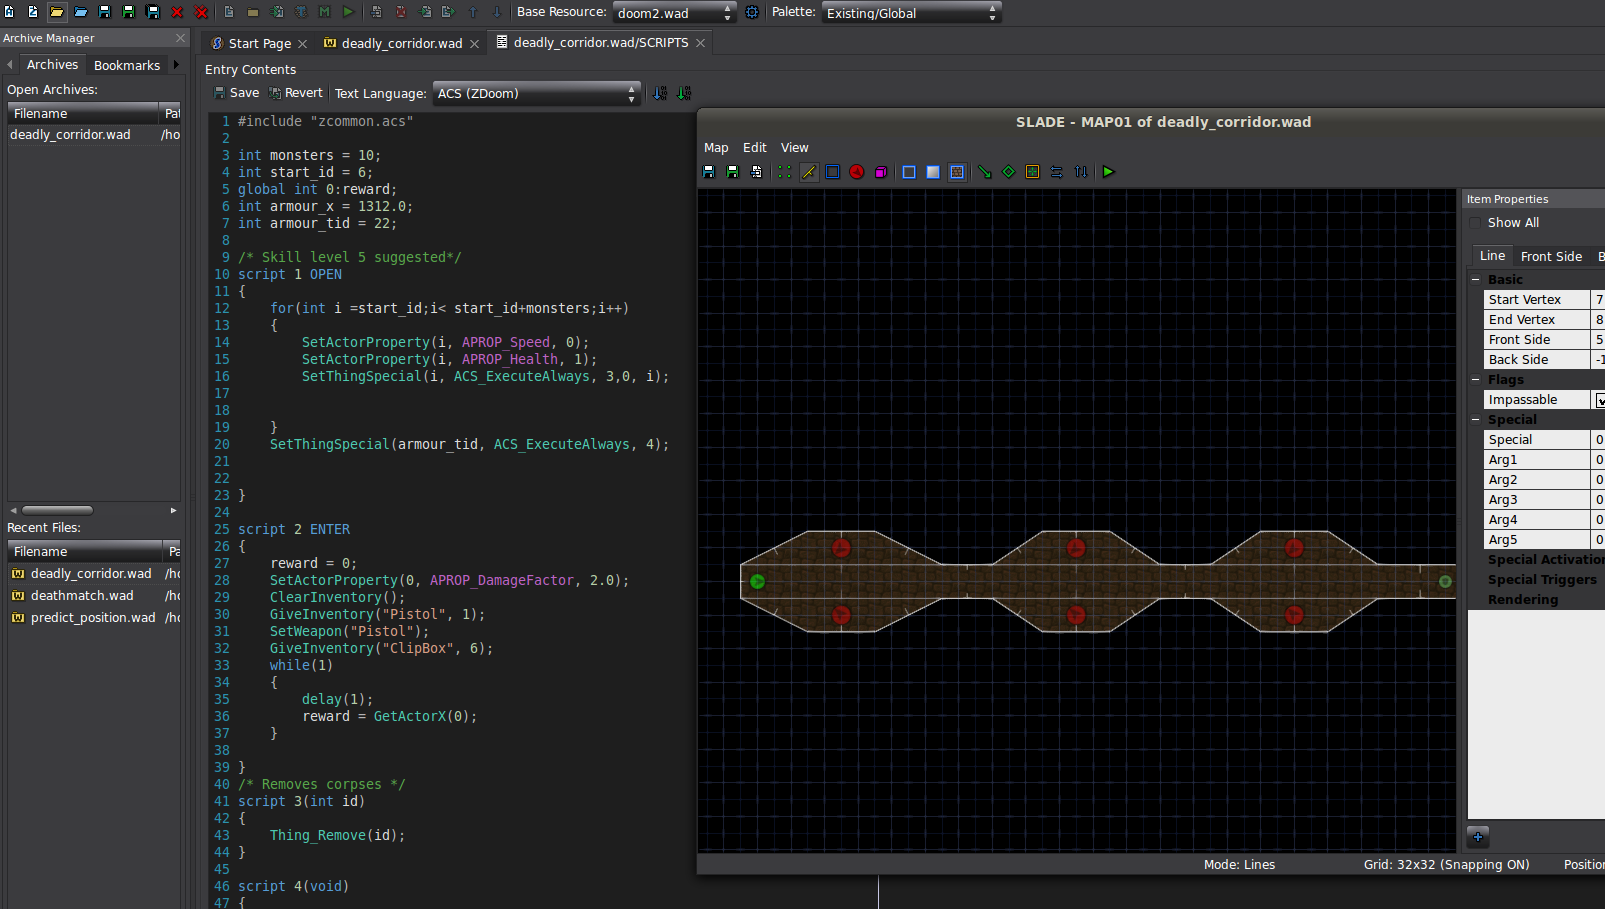
\includegraphics[scale=0.25]{slade.png}
			\caption{Slade 3 application for scenario creation.}\label{fig:slade}
	\end{figure}

	Creating WAD files involves compilation thus it~requires dedicated software. \emph{Slade~3} and \emph{Doom~Builder~2} were the editors of choice because of huge popularity, availability of resources and quality. The editors differ mostly in user interface details but~both provide most crucial functionalities:

	\begin{description}
		\item [Visual map editor] - a simple tool for map creation which is easy to use and~allows to build any imaginable map that Doom engine is capable of running.
		\item [Action Code Script support] - dedicated language resembling C that is suitable for regulating behaviors of monsters, players and~objects in the game.
		\item [Test running] - possibility to test a scenario without leaving the editor. Test running requires providing a \emph{zdoom} executive file and \emph{doom2.wad} file (or~any other basic resource file) . 
	\end{description}

	Both tools are robust, reasonably easy to use and~provide much elasticity in scenario creation, although neither program is free from serious user experience shortcomings. Nevertheless, they still remain superior to existing alternatives. Due to the lack of native \emph{Linux} support from \emph{Doom~Builder~2}, \emph{Slade~3} seems to be a more flexible solution. 

	\newpage
\section{Provided Scenarios}\label{sec:scenarios}
	This section describes ready-to-use scenarios that come with VIZIA.

	Each subsection includes `Suggested configuration' which suggests additional configuration which can be achieved by loading	configuration from a file (see Section \ref{sec:configuration_file}) or using additional API methods (see Section \ref{subsec:config_methods}). These particular configurations are quite arbitrary and adjusting them to personal preferences is encouraged.

	\subsection{Basic}\label{subsec:basic}
		
		\begin{figure}
			\centering
			\includegraphics[scale=0.46]{basic.png}
			\caption{Doom gameplay frame from `basic' scenario.}\label{fig:basic}
		\end{figure}

		\paragraph{Motivation}
			Main purpose of this scenario is to show that using VIZIA for Reinforcement Learning from visual input is a feasible idea. The scenario exposes most fundamental mechanics of the game like shooting, movement and delays between actions and reactions of the world.
		
		\paragraph{Description}
			The map is a rectangle with gray walls, ceiling and floor. Agent is spawned along the longer wall, in the center. A red, circular monster is spawned randomly somewhere along the~opposite wall. Agent can only (config) move left, move right and~shoot. A single hit is enough to kill the~monster. Episode ends when the monster is killed or on timeout.
		
		\paragraph{Rewards}
			\begin{itemize}
				\item +101 for killing the monster
				\item -5 for missing
			\end{itemize}
		
		\paragraph{Suggested configuration}
			\begin{itemize}
				\item living reward = -1
				\item available buttons: move left, move right, shoot (attack)
				\item timeout = 300
			\end{itemize}
	\newpage

	\subsection{Deadly Corridor}
		\begin{figure}
			\centering
			\includegraphics[scale=0.5]{deadly_corridor.png}
			\caption{Doom gameplay frame from `deadly corridor' scenario.}\label{fig:deadly_corridor}
		\end{figure}

		\paragraph{Motivation} 
			The purpose of this scenario is essentially to teach an agent to be a responsible adult with good spacial orientation: focus efforts towards a good direction and be able to sacrifice instant gratification in favor of future benefits and lifespan. Coping with the task requires some degree of spacial orientation and ability to see connection between monsters' presence and deteriorating health which, unattended, results in agent's death.

		\paragraph{Description}
			The map is a corridor with shooting monsters standing along the longer walls (6 monsters in total). Agent is spawned at one end of the corridor and a green vest is placed at the opposite one. Reward is proportional (negative or positive) to change of the distance between the agent and the vest. If agent ignores monsters on the sides and runs straight for the vest he will be killed somewhere along the way. To ensure this behavior \textit{doom\_skill} equal to 5 (config) is needed.

		\paragraph{Rewards}
			\begin{itemize}
				\item $\Delta$x for getting closer to(further from) the vest by $\Delta$x units in the corridor's axis of symmetry.
			\end{itemize}
			
		\paragraph{Suggested configuration}
			\begin{itemize}
				\item available buttons: turn left, turn right, move left, move right, shoot (attack)
				\item timeout = 4200
				\item death penalty = 100
				\item doom skill = 5
				\item available game variables: HEALTH
			\end{itemize}
	\newpage

	\subsection{Defend the Center}\label{subsec:defend_the_center}
		\begin{figure}
			\centering
			\includegraphics[scale=0.5]{defend_the_center.png}
			\caption{Doom gameplay frame from `defend the center' scenario.}\label{fig:defend_the_center}
		\end{figure}
		\paragraph{Motivation} 
			The purpose of this scenario is to encourage agents to develop some intuition about distances and awareness of potential dangers coming from behind. Obviously, agents should also learn that monsters are sinister and killing them is rewarding, but it is not sufficient. Coincidentally an agent could be expected to learn to impersonate a classical Greek tragic hero: he is doomed to die pitifully (ammunition is finite) regardless of his actions.

		\paragraph{Description}
			The map is a large circle. A player is spawned in the exact center and is allowed to turn and shoot (config). 5 melee-only, monsters are spawned along the wall. Monsters are killed after a single hit. If slain, monsters respawn after some time. Episode ends when the player dies (it is inevitable because of limited ammunition supplies).

		\paragraph{Rewards}
			\begin{itemize}
				\item +1 for killing a monster
			\end{itemize}
		
		\paragraph{Suggested configuration}
			\begin{itemize}
				\item death penalty = 1
				\item available buttons: turn left, turn right, shoot (attack)
				\item available game variables: HEALTH, AMMO2(pistol ammo)
			\end{itemize}
	\newpage

	\subsection{Defend the Line}
		\begin{figure}
			\centering
			\includegraphics[scale=0.5]{defend_the_line.png}
			\caption{Doom gameplay frame from `defend the line' scenario.}\label{fig:defend_the_line}
		\end{figure}
		\paragraph{Motivation} 
			The purpose of this scenarios is to teach agents risk assessment and basic monster taxonomy by presenting them with monsters of two types: melee fighters and shooters. Agents should be able to recognize that shooters pose more immediate threat than melee monster (unless they are at point blank range). Obviously, agents should also learn that monsters are sinister and killing them is rewarding, however it is not sufficient to perform superbly.
		\paragraph{Description}
			The map is a rectangle. Player is spawned along the longer wall, in the center and is able to turn and shoot(config). 3 melee and 3 shooting monsters are spawned along the opposite wall. Monsters are killed after a single shot, at first. When slain, each monster is respawned after some time and can endure more damage than before. Episode ends when the player dies (it's inevitable because at some point monsters will be too tough to kill).
		\paragraph{Rewards}
			\begin{itemize}
				\item +1 for killing a monster
			\end{itemize}

		\paragraph{Suggested configuration}
			\begin{itemize}
				\item available buttons: move left, move right, shoot (attack)
				\item death penalty = 1
				\item available game variables: HEALTH, AMMO2(pistol ammo)
			\end{itemize}
	\newpage

	\subsection{Deathmatch}
		\begin{figure}
			\centering
			\includegraphics[scale=0.5]{deathmatch.png}
			\caption{4 Doom gameplay frames from `deathmatch' scenario.}\label{fig:deatchmatch}
		\end{figure}
		\paragraph{Motivation} 
	 		This scenario is a fully fledged fight for survival that hopefully requires quite sophisticated cognitive processes. Agent should be able to present effective understanding of many high level concepts as fleeing, surroundings awareness, hiding, camping, resupplying, navigation or changing weapons to survive and kill a significant number of monsters.

		\paragraph{Description}
			The map consists of a square room (hall) of considerable size and 4 small rooms (supply rooms) adjacent to each wall of the hall. 2 supply rooms contain significant quantity of medkits and armors. Other 2 contain (each one) a shotgun, chainsaw, plasma gun, chaingun, rocket launcher and ammunition needed for aforementioned weapons. Agent is spawned in random location inside the hall. After a very short period monsters start spawning in random locations of the hall. Monsters include shooters and melee brawlers. Agent is rewarded for killing monsters. Toughest monsters are less probable to appear and produce greater rewards.
		\paragraph{Rewards}
			\begin{itemize}
				\item +1/2/3/4/5/10 for killing a monster (exact value depends on monster type).
			\end{itemize}
		
		\paragraph{Suggested configuration}
			\begin{itemize}
				\item available buttons: all buttons corresponding movement, turning, shooting and weapon change 
				\item timeout = preferred finite value
				\item death penalty = 100
				\item available game variables: HEALTH, ARMOR and all variables connected with weapons and ammo
			\end{itemize}		
	\newpage

	\subsection{Health Gathering}
		\begin{figure}
			\centering
			\includegraphics[scale=0.5]{health_gathering.png}
			\caption{Doom gameplay frame from `health gathering' scenario.}\label{fig:health_gathering}
		\end{figure}
		\paragraph{Motivation}
			The purpose of this scenario is to teach an agent that every second of his life is precious and collecting things increases his life expectancy in this brutal world. The agent should be able to see that deteriorating health causes death and how walking into medkits influences his health. It is advisable to equip the agent with some kind of memory because medkits that are directly in front of agent's feet cannot be noticed. In case of developing consciousness agent could also deduce that there is a divine being in the skies that loves him and sends provisions to save him.

		\paragraph{Description}
			The map is a rectangle with green, acidic floor which hurts players periodically. Deadliness of acid depends on skill level. Agent is spawned in the exact center of the map and is able to turn and move forward (config).  Initially there are some medkits uniformly distributed over the map. New medkits fall from the skies periodically. A medkit heals some portion of player's health - to survive agent needs to pick them up. Episode finishes after player's death or on timeout.

		\paragraph{Suggested configuration}
		\begin{itemize}
			\item living reward = 1
			\item death penalty = 100
			\item available buttons: move left, move right, move forward
			\item timeout = 2100
			\item available game variable: HEALTH
		\end{itemize}
	\newpage

	\subsection{My Way Home}
		\begin{figure}
			\centering
			\includegraphics[scale=0.22]{my_way_home.png}
			\caption{6 Doom gameplay frames from `my way home' scenario.}\label{fig:my_way_home}
		\end{figure}
		\paragraph{Motivation} 
			The purpose of this scenario is to teach the agent how to navigate in a labyrinth-like environment and reach his ultimate goal (and learn what the goal actually is). Agent should learn to determine his position in the maze and to navigate accordingly.

		\paragraph{Description}
			The map is a series of small rooms interconnected with each other by short passages and a single dead end corridor. Each room has a different color. A green vest is placed in one of the rooms (the same room every time). Player is spawned in randomly chosen room facing a random direction. Episode ends when the vest is reached or on timeout.
		\paragraph{Rewards}

		\begin{itemize}
			\item +1 for reaching the vest
		\end{itemize}
		
		\paragraph{Suggested configuration}
		\begin{itemize}
			\item living reward = -0.0001
			\item available buttons: move left, move right, shoot (attack)
			\item timeout = 2100
		\end{itemize}
	\newpage

	\subsection{Predict Position}
		\begin{figure}
			\centering
			\includegraphics[scale=0.32]{predict_position.png}
			\caption{2 Doom gameplay frames from `predict position' scenario.}\label{fig:predict_position}
		\end{figure}
		\paragraph{Motivation} 
			The purpose of the scenario is to teach agents to synchronize missile weapon shots (involving a significant delay between shooting and hitting) with target movements. Agent should be able to shoot so that missile and monster meet each other.

		\paragraph{Description}
			The map is a rectangle room. Agent is spawned along the longer wall, in the center and is allowed to turn and shoot(config). A monster is spawned randomly somewhere along the opposite wall and walks between left and right corners along the wall. Player is equipped with a rocket launcher and a single rocket. Episode ends when the missile hits the monster (or a wall) or on timeout.
		\paragraph{Rewards}
		\begin{itemize}
			\item +1 for killing the monster
		\end{itemize}
		
		\paragraph{Suggested configuration}
		\begin{itemize}
			\item living reward =-0.0001
			\item available buttons: turn left, turn right, shoot (attack)
			\item timeout = 300
		\end{itemize}
	\newpage

	\subsection{Take Cover}
		\begin{figure}
			\centering
			\includegraphics[scale=0.5]{take_cover.png}
			\caption{Doom gameplay frame from `take cover' scenario.}
		\end{figure}
		\paragraph{Motivation} 
			The purpose of this scenario is to teach agents to link incoming missiles with their estimated lifespan. Agents should learn that being hit means a decrease in health and this in turn leads to death that is most undesirable. In effect agents should learn how to avoid missiles.

		\paragraph{Description}
			Map is a rectangle. Player is spawned along the longer wall, in the center. A couple of fireball-spitting monsters are spawned randomly somewhere along the opposite wall and try to kill the player with fireballs. The player has no weapon and can only move sideways (config). More monsters appear with time. Episode ends when player dies which is inevitable.

		\paragraph{Suggested configuration}
		\begin{itemize}
			\item living reward = 1
			\item death penalty = 100
			\item 2 available buttons: move left, move right
		\end{itemize}
	\newpage

\section{Creating scenarios}\label{sec:creating_scenarios}
	This section is not intended as a reference manual for Action Code Script (ACS) or map creation thus covers only subjects directly relevant to interfacing between Doom game engine and VIZIA.


	\subsection{Fixed Point Numbers}\label{subsec:fixed_point}
		ACS does not support floating point numbers, however fixed point numbers are implemented using integers. By adding a decimal point the compiler is force to treat \emph{int} variable as a fixed point number so for instance `1' will be treated as an integer whereas `1.0' as a fixed point numeral. Mixing integers and fixed point numbers is allowed but will produce unexpected results if performed unknowingly. For more detailed information consult Zdoom Wiki Webpage\cite{zdoom-wiki}.

	\subsection{Global Variables}\label{subsec:global_variable}
		ACS provides a special type of variables called \emph{global~variables} that are seen by VIZIA API as game variables (see Section \ref{subsec:gamevar}) named USER<X>. Global variables behave the same as ordinary variables but need to be declared in global scope and in a slightly different way:
		\begin{clinee}
global int <X>:reward;
		\end{clinee}
		Where <X> denotes the ordinal number of the variable.
		
	\subsection{Rewards}
		In order to support the rewarding mechanism, it is necessary to utilize global variable 0 in the ACS script. Name given to the variable does not matter. The value of the variable represents total reward accumulated throughout the whole episode so in order to give a reward for a specific action it is needed to increase global variable 0 by the desired value not to assign it. VIZIA treats the reward global variable as a fixed point number(see \ref{subsec:fixed_point}).

	\subsection{Advices}
		This section shows code snippets showing how we achieved some ACS scripting behaviors that may prove useful. The code snippets intend to be relatively self-explanatory and assume knowledge of the very basics of ACS scripting and capability of reading documentation to make sense of used functions. For documentation and more detailed information consult Zdoom Wiki Webpage\cite{zdoom-wiki}.

		\subsubsection*{Ending an Episode}

			\begin{clinee}
Exit_Normal(0);
			\end{clinee}
		\subsubsection*{Reward for Killing a Monster} This snippet is also useful for triggering any event after killing a monster or collecting an item.
			\begin{clinee}
script 123 (void)
{
	reward = reward + 1;
}
SetThingSpecial(MONSTER_TID, ACS_ExecuteAlways, 123);
			\end{clinee}
\subsubsection*{Friendly Monster}
			\begin{clinee}
Thing_Hate (MONSTER_TID, SOME_UNUSED_TID, 6);
			\end{clinee}
		\subsubsection*{Stationary Monster}
			\begin{clinee}
SetActorProperty(MONSTER_TID, APROP_Speed, 0);
			\end{clinee}
		\subsubsection*{Single Hit Monster}
			\begin{clinee}
SetActorProperty(MONSTER_TID, APROP_Health, 1);
			\end{clinee}
		\subsubsection*{Self-replenishing Ammo}
		Note that this can also be achieved by changing Zdoom's configuration but these changes are persistent.
			\begin{clinee}
script 2 ENTER
{   
    while(1)
    {
        delay(1);
        GiveInventory("Clip", 1 );
    }
}
			\end{clinee}
		\subsubsection*{Disappearing Corpses}
			\begin{clinee}
script 234 (int TID)
{
	Thing_Remove(TID);
}
SetThingSpecial(MONSTER_TID, ACS_ExecuteAlways, 234, MONSTER_TID);
			\end{clinee}

\chapter{Reinforcement Deep Learning Experiment}\label{ch:experiment}

\section{Goal of the Experiment}
The main purpose of the experiment is to show that reinforcement learning from visual input is possible using VIZIA Environment. 	
Additionally, the experiment tries to investigate how skipping varying number of frames influences learning process.

\section{Experiment's Design}
During the experiment, agents with varying \emph{skiprates} are to be tested. We define \emph{skiprate} as the number of game frames that are skipped(ignored) by agent for every frame that is processed. Skipping a frame is accomplished with \emph{makeAction} method with tics argument set to skiprate (see Section \ref{subsec:runtime_methods}) so rewards are accumulated and the chosen action is extended for the duration of skipped frames. Skiprate values of 0,1,2,3,4,5~and~7 are evaluated in the experiment. 

Every agent is to run 80 epochs. Each epoch requires performing 5000 learning steps that involve performing an action (observing a transition) and running a learning update. After the learning portion of each epoch, 100 random test episodes are conducted and mean score is used for assessment.  

\section{Tested Agent's Design}
	The agent is heavily inspired by Google DeepMind Atari DQN \cite{mnih-dqn-2015}\cite{mnih-atari-2013} and is conceptually very similar to the aforementioned algorithm. Game is modeled as a Markov Decision Process and Q-learning \cite{watkins:mlj92} is used to reach the optimal policy. $\epsilon$-greedy policy with linear $\epsilon$ decay is used to choose actions. Additionally, a technique called experience replay \cite{mnih-dqn-2015} is applied. A state is represented by only the most recent image therefore agents have no memory. A Convolutional Neural Network is used for approximation of Q-values and it is trained with Backpropagation Algorithm \cite{lecun-98b} using Stochastic Gradient Descent with mini-batches. An agent is implemented in Python and uses Theano \cite{Bastien-Theano-2012}\cite{bergstra+al:2010-scipy} and Lasagne \cite{sander_dieleman_2015_27878} libraries for neural networks. Neural network's forward and backward passes are computed on GPU whereas the rest of the code runs on the CPU.

\newpage
\section{Experimental Setup} 
	\subsection{Operating System and Hardware}
	\begin{description}
		\item[Operating System] Linux Mint 17 x86\_64, kernel 3.13.0-24-generic
		\item[CPU] Intel Core i7-4790, 4x4GHz
		\item[GPU] GeForce GTX 970, 1664 CUDA cores, 4GB RAM
	\end{description}

	\subsection{Game Settings}
		The experiment uses the simplest scenario from the pool, that is the `basic' scenario (see \ref{subsec:basic}). State is represented by 3-channel image (RGB) with resolution of 60 by 45 pixels.

	\subsection{Neural Network Architecture}
		\begin{figure}
			\centering
			\includegraphics[scale=0.25]{net_diagram.png}
			\caption{Schematic illustration of neural network used for the experiment.}\label{fig:network}
		\end{figure}
		 The network used in the experiment consists of two convolutional layers with 32 square filters (7 and 4 pixels wide) each connected to a max-pooling layer with poolsize equal to 2 and rectifier linear units. Convolutional layers are followed by a fully connected layer with 800 leaky rectified linear units and output layer with 8 linear units corresponding to 8 available actions (combinations of 3 available buttons). The architecture used is rather modest, compared to the ones used for other tasks recently.
	
	\subsection{Hyper Parameters}
		\begin{itemize}
		\item $\gamma$ (discount factor) = 0.99
		\item learning rate = 0.01
		\item mini-batch size = 40
		\item initial $\epsilon$ = 1.0
		\item final $\epsilon$ = 0.1
		\item steps after which $\epsilon$ decay will start = 100000
		\item steps to fully decrease $\epsilon$ = 100000
		\item replay memory  capacity = 10000
		\end{itemize}
	

\section{Results}
		\begin{figure}
			\centering
			\includegraphics{results.png}
			\caption{Graphs showing mean performance of tested agent with different skip values throughout 80 learning epochs.}\label{fig:results}
		\end{figure}
	\subsection{Numerical Issues}
		In case of 0 skiprate a major numerical problem was encountered. Estimated Q-values usually ($\approx$50\% of runs) rapidly grew to infinite values (in the first epoch) which prevented further learning. Quite unexpectedly, increasing resolution from 60x45 to 120x90 eliminated the problem at the cost of longer learning time. Faulty code would be an obvious explanation, however no apparent error has been found yet therefore a conceptually oriented mechanism is also to be considered. It is hypothesized that combination of zero skiprate and low resolution may produce state transitions that incorporate barely distinguishable states. As a consequence each update would significantly inflate Q-values for each state and rapidly reach infinity. Although changing the resolution seemed to solve the problem, it is not a satisfying solution and one based on mechanics of Q-learning itself would be much more desirable.

		Skiprate 0 setting was tested for both resolutions, however the agent with increased resolution was considered separately (see Figure \ref{fig:results_skiprate0}). Due to high number of epochs required to get fairly satisfying results with zero skiprate and increased resolution, learning was continued for further 270 epochs to see if it would follow the trend as expected.

	\subsection{Learning Quality}
		As seen in Figure \ref{fig:results}, all agents reached estimated maximum average score of $\approx$80 or showed trend towards achieving similar value. Watching agents play the scenario proved that agents in fact behave very reasonably. They move towards the target and shoot when it appears in front of them. Occasionally agents fire marginally too soon or stay idle (first available action) throughout whole episode. 
		
	\subsection{Skiprate Influence}
			
			
		\subsubsection*{Learning speed} 

			\begin{table}
				\begin{center}
					\begin{tabular}{ |c | c |}
						\hline
						Skiprate & Average epoch duration [s] \\ \hline
						0 & 51.79 \\ \hline
						1 & 51.83 \\ \hline
						2 & 52.84 \\ \hline
						3 & 53.84 \\ \hline
						4 & 52.88 \\ \hline
						5 & 53.15 \\ \hline
						7 & 53.12 \\ \hline
					\end{tabular}
				\end{center}
				\caption{Influence of skiprate on processing time for resolution of 60X45}\label{tab:time_results}
			\end{table}
			As seen in the Figure \ref{fig:results} higher skiprate leads to quicker (in terms of learning steps) and smoother learning, which was expected as higher skiprate makes consequences of actions more immediate and easier to notice. However, it must be pointed out that epoch's duration slightly increases with raising skiprate (see Table \ref{tab:time_results}). Obviously, such behavior was anticipated because Doom engine has to process skiprate as many frames (which we skip) for a single learning step (action). Additionally, higher skiprate results in episodes being shorter (because we skip most of frames) which increases overhead associated with episode restarts (restarts are more frequent). 

		\subsubsection*{Score}
			\begin{table}
				\begin{center}
					\begin{tabular}{ |l || c | r |}
						\hline
						Skiprate & Best epoch score & Mean of 10 best epochs \\ \hline
						0 & 69.18 $\pm$ 50.24 & 60.97 \\ \hline
						1 & 77.84 $\pm$ 22.71 & 76.19 \\ \hline
						2 & 79.35 $\pm$ 20.68 & 77.91 \\ \hline
						3 & 80.98 $\pm$ 22.89 & 78.69 \\ \hline
						4 & 81.8 $\pm$ 17.99 & 80.75 \\ \hline
						5 & 81.32 $\pm$ 19.47 & 80.16 \\ \hline
						7 & 81.08 $\pm$ 18.9 & 80.5 \\ \hline
					\end{tabular}
				\end{center}
				\caption{Influence of skiprate on highscores achieved in 80 epochs.}\label{tab:results}
			\end{table}
			It was also anticipated that higher skiprate could slightly lower scores due to the lack of small-grained control. As seen in Table \ref{tab:results}, it is exactly the opposite. It is doubtful whether too short training is the culprit of this trend, since most of agents reach significant stability in 80 epochs and do not appear to be able to ever transcend achieved highscores (at least for skiprates $\geq$ 2). What is more, it was observed that agents with higher skiprates were less prone to irrational behaviors like staying idle or going the opposite way which may coincide with much smoother learning. However, it is hypothesized that careful fine-tuning of hyper parameters could positively influence learning rate and smoothness. 

			Learning process was especially fuzzy for zero skiprate with increased resolution (see Figure \ref{fig:results_skiprate0}) but it appears that it was slowly converging to the optimum and intensity of occasional terrible-performance episodes was fading. Further learning (preferably with lowered learning rate) would be necessary to confirm the hypothesis.
	
	\begin{figure}
		\centering
		\includegraphics{results_skiprate0.png}
		\caption{Graphs showing mean performance of agent with zero skiprate and resolution 120x90 throughout 350 learning epochs.}\label{fig:results_skiprate0}
	\end{figure}

	


\chapter{Conclusions}

\section{Achieved Goals}
\section{Future Work}



% Bibliography (books, articles) starts here.
\bibliographystyle{plain}{\raggedright\sloppy\small\bibliography{bibliography}}

% All appendices and extra material, if you have any.
\cleardoublepage\appendix%

\chapter{GitHub}
The thesis and VIZIA framework are available on the github server: \\
\url{https://github.com/Marqt/Vizia/} 


\chapter{Building}
\section{Prerequisites}
\begin{itemize}
\item preferably Linux
\item cmake
\item make
\item gcc 4.??
\item Boost 
\item Python 2.6+ with Numpy and Boost.Python (for pyhon binding)
\item Java compiler (for Java binding)
\end{itemize}
\section{Before Building}
	In addition to prerequisites mentioned above, the following packages need to be install to build Zdoom itself:
	\begin{description}
		\item[Debian/Ubuntu:] \hfill \\
		sudo apt-get install build-essential zlib1g-dev libsdl2-dev libjpeg-dev nasm tar libbz2-dev libgtk2.0-dev cmake git libfluidsynth-dev libgme-dev libopenal-dev timidity
		\item[Fedora:] \hfill \\
		yum install gcc-c++ make zlib-devel SDL2-devel libjpeg-turbo-devel nasm tar bzip2-devel gtk2-devel cmake git fluidsynth-devel game-music-emu-devel	openal-soft-devel timidity++
		\item[Arch linux:] \hfill \\
		pacman -S --needed gcc make zlib sdl2 libjpeg-turbo nasm tar bzip2 gtk2 cmake git fluidsynth libgme fmodex openal timidity++
		\item[openSUSE:] \hfill \\
		zypper install gcc-c++ make zlib-devel libSDL2-devel libjpeg-devel nasm tar libbz2-devel gtk2-devel cmake git fluidsynth-devel libgme-devel openal-soft-devel timidity
	\end{description}
\section{Compilation}
To compile Vizia run this commands 
	\begin{lstlisting}
cmake -DCMAKE_BUILD_TYPE=Release
make all
	\end{lstlisting}
\chapter{Methods and Structures Handout}
\section{Methods}
\section{Structures and Enumerations}\label{sec:appendix_structs_and_enums}


% Colophon is a place where you should let others know about copyrights etc.
\ppcolophon

\end{document}
